\documentclass[finnish]{tktltiki2}

% tktltiki2 automatically loads babel, so you can simply
% give the language parameter (e.g. finnish, swedish, english, british) as
% a parameter for the class: \documentclass[finnish]{tktltiki2}.
% The information on title and abstract is generated automatically depending on
% the language, see below if you need to change any of these manually.
% 
% Class options:
% - grading                 -- Print labels for grading information on the front page.
% - disablelastpagecounter  -- Disables the automatic generation of page number information
%                              in the abstract. See also \numberofpagesinformation{} command below.
%
% The class also respects the following options of article class:
%   10pt, 11pt, 12pt, final, draft, oneside, twoside,
%   openright, openany, onecolumn, twocolumn, leqno, fleqn
%
% The default font size is 11pt. The paper size used is A4, other sizes are not supported.
%
% rubber: module pdftex

% --- General packages ---

\usepackage[utf8]{inputenc}
\usepackage[T1]{fontenc}
\usepackage{lmodern}
\usepackage[pdftex]{graphicx}
\usepackage{subfigure}
\usepackage{microtype}
\usepackage{amsfonts,amsmath,amssymb,amsthm,booktabs,color,enumitem,graphicx}
\usepackage[pdftex,hidelinks]{hyperref}

% Automatically set the PDF metadata fields
\makeatletter
\AtBeginDocument{\hypersetup{pdftitle = {\@title}, pdfauthor = {\@author}}}
\makeatother

% --- Language-related settings ---
%
% these should be modified according to your language

% babelbib for non-english bibliography using bibtex
\usepackage[fixlanguage]{babelbib}
\selectbiblanguage{finnish}

% add bibliography to the table of contents
\usepackage[nottoc]{tocbibind}
% tocbibind renames the bibliography, use the following to change it back
\settocbibname{Lähteet}

% --- Theorem environment definitions ---

\newtheorem{lau}{Lause}
\newtheorem{lem}[lau]{Lemma}
\newtheorem{kor}[lau]{Korollaari}

\theoremstyle{definition}
\newtheorem{maar}[lau]{Määritelmä}
\newtheorem{ong}{Ongelma}
\newtheorem{alg}[lau]{Algoritmi}
\newtheorem{esim}[lau]{Esimerkki}

\theoremstyle{remark}
\newtheorem*{huom}{Huomautus}


% --- tktltiki2 options ---
%
% The following commands define the information used to generate title and
% abstract pages. The following entries should be always specified:

\title{Digitaaliset todennukset mobiiliympäristössä}
\author{Taneli Virkkala}
\date{\today}
\level{Kandidaatin tutkielma}
\abstract{Mobiililaitteiden teknologinen kehitys on mahdollistanut monien viestien vaihtoon soveltuvien protokollien käytön nykypäivänä. Näihin protokolliin kuuluu laitteen käyttäjän todennus, viestin lähettäjän todennus, viestin datan eheys ja saapuminen oikealle vastaanottajalle. Digitaalinen allekirjoitus, MAC-funktio sekä Diffien ja Hellmanin menetelmä mahdollistavat turvallisen viestien vaihton kahden osapuolen välillä.

Mobiililaite koostuu SIM-kortista ja prosessorista. Digitaaliseen allekirjoitukseen tarvittavaa avainta voidaan säilyttää laitteen muistissa tai SIM-kortilla. Digitaalisen allekirjoituksen voi tehdä kokonaan laitteen avulla tai delegoida operaation palvelimelle. Palvelimelle on hyvä luoda turvattu VPN-yhteys, jossa kaikki tieto voi kulkea salattuna.

Luotettavaan tietoturvaan kuuluu lisäksi käyttäjän todentaminen mobiililaitteelle. Koska todentamisen tulee olla nopeaa, tehokkuus on otettava huomioon protokollien käytössä.}

% The following can be used to specify keywords and classification of the paper:

\keywords{mobiiliympäristö, digitaalinen todennus, digitaalinen allekirjoitus, MAC-funktio, RSA, Diffie-Hellman}

% classification according to ACM Computing Classification System (http://www.acm.org/about/class/)
% This is probably mostly relevant for computer scientists
% uncomment the following; contents of \classification will be printed under the abstract with a title
% "ACM Computing Classification System (CCS):"
\classification{C.2.1 [Wireless communication]\newline E.3 [Public key cryptosystems]\newline K.6.5 [Authentication]}

% If the automatic page number counting is not working as desired in your case,
% uncomment the following to manually set the number of pages displayed in the abstract page:
%
% \numberofpagesinformation{16 sivua + 10 sivua liitteissä}
%
% If you are not a computer scientist, you will want to uncomment the following by hand and specify
% your department, faculty and subject by hand:
%
% \faculty{Matemaattis-luonnontieteellinen}
% \department{Tietojenkäsittelytieteen laitos}
% \subject{Tietojenkäsittelytiede}
%
% If you are not from the University of Helsinki, then you will most likely want to set these also:
%
% \university{Helsingin Yliopisto}
% \universitylong{HELSINGIN YLIOPISTO --- HELSINGFORS UNIVERSITET --- UNIVERSITY OF HELSINKI} % displayed on the top of the abstract page
% \city{Helsinki}
%


\begin{document}

% --- Front matter ---

\frontmatter      % roman page numbering for front matter

\maketitle        % title page
\makeabstract     % abstract page

\tableofcontents  % table of contents

% --- Main matter ---

\mainmatter       % clear page, start arabic page numbering

\section{Johdanto}

% Write some science here.


Digitaalisten todennusten käyttö on kasvanut huomattavasti mobiililaitteilla nykypäivänä. Mobiiliympäristössä turvallinen yhteys on varmistettava, koska tietoturvariskit langattomissa verkoissa ovat erittäin suuret \cite{enti}. Teknisen kehityksen ansiosta todennuksia voidaan hyödyntää yleisesti mobiililaitteilla, ja parempi tietoturva on mahdollistanut useiden sovellusten käytön. Tietokonelaitteistolla käytettävät menetelmät, kuten esimerkiksi PKI-malli (julkisen avaimen infrastruktuuri), ovat siirtyneet mobiiliympäristöön sellaisenaan, eivätkä nämä mallit ole tarvinneet suuria muutoksia toimiakseen. Kehittyneemmän laskentatehon ansiosta monet algoritmit, kuten RSA digitaalisessa allekirjoituksessa sekä Diffien ja Hellmanin menetelmä, on pystytty ottamaan käyttöön kannettavilla laitteilla \cite{enti}. Yhteiseen salaisuuteen perustuva MAC-funktio on myös käytössä tekstiviestien (SMS) lähettämisessä \cite{MAC} ja salausavainten luomisessa \cite{MACA}. Operaatiot, joita laitteella ei pystytä suorittamaan, voidaan delegoida palvelimille. Allekirjoitus voidaan luoda tarvittaessa palvelimella tai asiakkaan laitteessa, mutta allekirjoituksen tulee täyttää kaikki sille asetetut tietoturvaehdot. Palvelinpohjaisen allekirjoituksen yleensä luo välissä oleva kirjautumispalvelin eikä lopullinen palveluntarjoaja \cite{proxy}. Palvelimelle voidaan luoda turvallinen VPN-yhteys, jossa kaikki tieto kulkee salattuna käyttäjän ja vastaanottajan välillä \cite{vpn}.

Digitaalisten todennusten käyttö tulisi mobiiliympäristössäkin  olla nopeaa ja turvallista. Digitaalinen allekirjoitus on turvallisin tapa varmentaa käyttäjä, sillä menetelmään kuuluu viestin lähettämisen kiistämättömyys. Monet nykyaikaiset sovellukset vaativat jokaisen viestin lähetyksen yhteydessä uuden allekirjoituksen. On siis luotava allekirjoitus nopean ajan sisällä tietoturvasta karsimatta. Esimerkkinä tästä voisi toimia eräänlainen huutokauppasovellus, jossa jokaisen huudon on oltava kiistaton ja todennettu \cite{proxy}. Lisäksi viestin sisältämän datan tulee olla eheää ja varmennettu. Varmenne on varmenneviranomaisen tarjoama osa digitaalisen allekirjoituksen luontiin. Jokainen allekirjoitus tarvitsee varmenteen, jonka lähettäjä liittää allekirjoitukseen \cite{ECC}.   

Schwabin ja Yangin mukaan \cite{enti} mahdollisiin tietoturvariskeihin mobiiliympäristössä liittyy urkinta, välimieshyökkäys, datan muuntaminen, toisena osapuolena esiintyminen ja laitteen kadottaminen. Mobiililaitteen sisäisen toiminnan ja verkkoviestinnän tulee olla suojattu mahdollisilta riskeiltä. Jos palvelun tarjoajan ja asiakkaan välissä on välityspalvelin, siihen tulee myös muodostaa luotettava yhteys. Koska digitaaliset allekirjoitukset perustuvat julkisen avaimen infrastruktuuriin, on äärimmäisen tärkeää pitää salainen avain mahdollisimman turvassa. Laitteen SIM-kortti on turvallinen paikka säilyttää salaista avainta, joka ei silloin paljastu laitteen käyttöjärjestelmälle. Sen sijaan prosessorilla avaimen ja allekirjoituksen luonti on nopeampaa kuin SIM-kortilla, mutta silloin käyttöjärjestelmä näkee laitteen prosessorin luoman avaimen kokonaan \cite{proxy}.        


\section{Digitaaliset todennukset}

Digitaalisiin todennuksiin kuuluvat epäsymmetristä todennusta käyttävä digitaalinen allekirjoitus ja muut julkisen avaimen infrastruktuuriin pohjautuvat menetelmät. Lisäksi todennuksiin voidaan luetella symmetristä salausta käyttävät protokollat. Symmetrisiä tapoja todentaa ovat yhteiseen salaisuuteen perustuvat Diffien ja Hellmanin menetelmä sekä MAC-funktio. Kaikkien todennusten on täytettävä seuraavat kriteerit: viesti on lähtenyt oikealta lähettäjältä, viesti on saapunut muuttumattomana perille ja vain vastaanottaja pystyy lukemaan viestin. Vastaanottaja pystyy kuitenkin muuttamaan viestiä saatuaan sen tai kiistämään viestin saapumisen perille.

\subsection{Historia}

RSA algoritmina kehitettiin jo vuonna 1977. Ron Rivest, Adi Shamir ja Leonard Adleman \cite{rsa78} keksivät julkisen avaimen infrastruktuuriin pohjautuvan menetelmän, jossa salaus hoidetaan julkisella avaimella ja viestin purkaminen salaisella avaimella. Tätä salausmuotoa kutsutaan epäsymmetriseksi salaukseksi erillisten avainten takia. Vain vuotta aikaisemmin Whitfield Diffie ja Martin Hellman \cite{dh76} loivat Diffien ja Hellmanin menetelmän (DH), joka mahdollisti kahden osapuolen viestien salauksen. DH luo osapuolille yhden yhteisen avaimen, jolla viestit sekä salataan että puretaan. Samalla avaimella salaaminen ja purkaminen tarkoittaa symmetristä salausta. Käyttötarkoitus DH:ssa on vain erilainen. RSA:ta käytetään digitaalisen allekirjoituksen luontiin, mutta DH perustuu käyttäjien viestien salaamiseen (symmetrinen salaus) ilman erillistä allekirjoitusta. Tämä kyseinen salaisuus DH:ssa voidaan sopia julkisia yhteyksiä pitkin, mutta lopputuloksena vain kaksi osapuolta saavat tietää tämän salaisuuden. DH:ssa viestin salaus ja purku tehdään samalla avaimella, josta on kopio kummallakin käyttäjällä.

Vuonna 1988 luotiin tarkat vaatimukset digitaalisille allekirjoituksille. Goldwasserin, Micalin ja Rivestin \cite{siam} mukaan allekirjoitukset eivät saa noudattaa mitään selkeää kaavaa, josta selväkielinen teksti saataisiin yhdistettyä salattuun tekstiin. Julkinen avain voi olla hallussa ulkopuolisella hyökkääjällä, jolla hän purkaa salatut tekstit ja pystyy päättelemään allekirjoituksen rakenteen tuleville viesteille. DH:n aikana vuonna 1976 oli käytössä takaporttifunktio, joka oli vielä turvattomampi \cite{dh76}. Jo pelkällä avaimen hallussapidolla kuka tahansa pystyi satunnaisella todennäköisyydellä luomaan pätevän tiivisteen viestille. Lyhyellä viestillä $M$ ja julkisella avaimella $k$ hyökkääjä pystyi verifioimaan lyhyen viestin, jolloin hän pääsi lähettämään ja purkamaan yksinkertaisia sanomia. Tiivisteitä ei ollut siis DH:n ensimmäisessä versiossa vielä käytössä.

Internetin laajentuessa ympäri maailmaa 1990-luvun alkupuolella monet sähköiset palvelut yleistyivät. Netscapen kehittämä SSL-protokolla vuonna 1995 oli alku myös myöhemmin käyttöön tulleelle TLS:lle. Nämä kummatkin protokollat toivat salauksen Internet-yhteyden välillä toimiviin sovelluksiin. Esimerkiksi HTML-sivujen siirrossa voidaan käyttää turvallista HTTPS-protokollaa, jossa data kulkee salatussa muodossa. Salaus ja purku voivat noudattaa PKI-mallia käytettäessä TLS:llää. Suomessa keksitty SSH-protokolla mahdollisti puolestaan etäyhteyden asiakkaan ja palvelimen välillä TCP-yhteydessä \cite{bulk}. Allekirjoitusalgoritmit kuten RSA tulivat tämän kaltaisessa yhteyden muodostuksessa yleisiksi ja salaisella avaimella voitiin korvata salasanalla tunnistautuminen. Nykyisin myös mobiililaitteella voi muodostaa etäyhteyksiä, ja aivan samoja TLS- ja HTTPS-protokollia käytetään osapuolten todennuksissa mobiilisovelluksissa.

2000-luvun alussa digitaaliset allekirjoitukset yleistyivät mobiililaitteissa. WAP-sovellusten (Wireless Application Protocol) tullessa käyttöön digitaalisia todennuksia pystyttiin käyttöönottaa mobiiliympäristössä ja monet yritykset alkoivat todentaa asiakkaitaan mobiiliallekirjoituksilla. Suomessa vasta vuonna 2010 kehitettiin mobiilivarmennejärjestelmä, johon mobiiliverkko-operaattorit lähtivät mukaan \cite{mobiva}. Virossa jo vuonna 2007 käynnistyi M-ID tunnistautuminen, jossa kansalainen pääsee käyttämään sähköisiä palveluita todentamalla henkilöllisyytensä matkapuhelimeltaan \cite{estonia}. 


\subsection{Digitaalisen allekirjoituksen määritelmä}

Digitaalinen allekirjoitus on menetelmä, jolla voidaan todentaa tietyn lähettäjän lähettäneen viestin vastaanottajalle muuttumattomana. Lähettäjä ei voi siis jälkikäteen kiistää lähettämäänsä viestiä (kiistämättömyys). Viesti voi olla lisäksi salattu käyttäen jotain salausmenetelmää kuten esimerkiksi AES-lohkosalausta. Vaikka viestin salaaminen ei suoranaisesti liity digitaaliseen allekirjoitukseen, on salaus tärkeä osa tietoturvaa. Digitaalinen allekirjoitus pohjautuu julkisen avaimen infrastruktuuriin, jossa käytetään kahta eri avainta. Toista käytetäään tiivisteen salaamiseen (allekirjoittaminen) ja toista tiivisteen purkamiseen. Allekirjoitus vaatii toimiakseen tiivistefunktioita ja varmenteen varmenneviranomaiselta. Viesti on siis saapunut oikeana perille, mikäli viestin tiiviste on sama kuin allekirjoitettu tiiviste. Mobiiliallekirjoituksella puolestaan tarkoitetaan digitaalista allekirjoitusta mobiililaitteella. Allekirjoituksen toimintaperiaate on mobiililaitteella ja tietokonelaitteistolla samanlainen.

\subsection{Digitaalisen allekirjoituksen toiminta} 

Tiivisteistä ja datan eheydestä voidaan todentaa tiedon muuttumattomuus ja lähettäjän kiistämättömyys \cite{moen}. Vastaanottaja purkaa viestin allekirjoituksen allekirjoittajan lähettämällä julkisella avaimella eli purkaa allekirjoitetun tiivisteen salauksen. Lisäksi viestistä tulee laskea tiiviste ennalta sovitulla tunnetulla tiivistefunktiolla. Molempien tiivisteiden arvojen tulisi olla samat, jotta viesti voidaan hyväksyä. Vastaanottaja vertaa viestistä laskettua tiivistettä ja purettua allekirjoitettua tiivistettä keskenään (verifionti). Jos viestin sisältöä muutetaan, viestistä laskettu tiiviste ei ole enää sama julkisella avaimella puretun tiivisteen kanssa. Ulkopuolisen hyökkääjän muutokset viestiin vaikuttavat tiivisteeseen ja tiivisteen arvaaminen päteväksi kestäisi vuosia. Tiivistefunktioina voidaan käyttää SHA-2 ja MD5. On syytä huomata, että SHA-1 ja MD5 ovat jo vanhentuneita tietoturvan kannalta ja uusi standardi SHA-3 on tuloillaan \cite{nist}.   

Viestin varmenteessa on mukana lähettäjän liittämä julkinen avain, jollei sitä ole lähetetty aiemmin. Varmenteen kelpoisuus on varmistettava varmenneviranomaiselta. Myönnetty varmenne on voimassa vain tietyn aikaa, joten voimassaolo on tarkistettava. Vastaanottajan on tunnettava kyseinen varmenneviranomainen viestin kelpoisuuden tarkastamiseksi. Kelpoisuus on siis tarkastettava viranomaisen julkisella avaimella, joka on saatettu lähettää saman viestin mukana. Seuraavien ehtojen on oltava voimassa allekirjoituksessa: uskottavuus, muuttumattomuus, uudelleenkäyttämättömyys ja kiistattomuus \cite{e-c}. Digitaalisella allekirjoituksella voidaan siis todentaa vain yksi viesti kerrallaan, ja jokaiselle viestille on luotava uusi allekirjoitus. Menetelmä on yksi turvallisimmista tavoista varmentaa luotettava viestinkulku kahden osapuolen välillä. Sen sijaan allekirjoitus on raskasta luoda, joten menetelmä vaatii merkittävää laskentatehoa toimiakseen \cite{proxy}. Erityisen vaikeaksi tekee tilanne, jossa salausta joudutaan käyttämään joka palvelimelle siirryttäessä. Digitaalisia allekirjoituksia käytetään siis yleensä yhteydenmuodostuksen aluksi osapuolten todentamiseen, mutta niistä voidaan luopua myöhemmissä viestien lähetyksissä.

\subsection{Matemaattisia selityksiä}

Algoritmien tulkinta vaatii pohjaksi tietämystä matemaattisista funktioista. Kongruenssirelaatiota käytetään monissa kaavoissa, joissa käytetään modulaarista aritmetiikkaa. Kongruenssirelaatio eli merkki $\equiv$ tarkoittaa kahden luvun $b$ ja $c$ erotuksen jaollisuutta luvulla $m$. Laskusta $(b - c)/m$ täytyy tulla lopputulokseksi kokonaisluku. Voidaan siis merkitä $b \equiv c \pmod{m}$, josta saadaan tulokseksi aina 0. Todetaan siis luvun $b$ olevan kongruentti $c$:n kanssa $\pmod{m}$. Esimerkiksi luku 6 on kongruentti 9 $\pmod{3}$. Merkitään 6 $\equiv $ 9$ \pmod{3}$, koska 6 - 9 $\pmod{3}$ = -3 $\pmod{3}$ eli 0. \cite{cong}

Keskenään jaottomien lukujen (suhteellinen alkuluku) idea perustuu siihen, että toista lukua ei voi päätellä toisesta jakojäännösten perusteella. Tämä sama sääntö pätee myös potenssiin korotuksissa. Oletetaan lukujen $p$ ja $q$ olevan alkulukuja. Niiden suurin yhteinen tekijä (syt) on siten 1. Koska syt$(p, q)$ = 1, niin positiivisilla eksponenteilla $m$ ja $n$ tämä sääntö ei muutu. Voidaan todeta siis aina alkuluvulla itsellään kertomisen säilyttävän suurinpana yhteisenä tekijänä luvun 1 eli syt$(p^m, q^n)$ = 1. \cite{rel}  

RSA:ssa käytettävä Eulerin funktio eli $\phi(n)$ kertoo niiden positiivisten kokonaislukujen $k$ lukumäärän ehdolla $1 \leq k \leq n$, joiden suurin yhteinen tekijä $n$:nän kanssa on 1. Eli luku $k$ ja luku $n$ ovat tällöin suhteellisia alkulukuja keskenään. Esimerkiksi $\phi(12) = 4$ sillä lukujen 1,5,7 ja 11 ainoa yhteinen tekijä luvun 12 kanssa on 1. Jos kyseessä on alkuluku $p$, sille on olemassa aina  keskenään jaottomia lukuja $p - 1$ verran. Voidaan todeta $\phi(p) = p -1$. Eulerin funktiolla saadaan tulokseksi lukujoukko, josta saadaan tarvittavat tekijät avainpareihin RSA:ssa. \cite{tot}
	
Primitiivijuuri tarkoittaa, että kokonaisluku $g$ potenssiin $n$ ja jakojäännös alkuluvusta $p$ ehdoilla $1 \leq n \leq p$ tuottaa kaikki kokonaisluvut väliltä 1 ja $p-1$. Kyseessä on $\phi(p) = p - 1$ määrän verran lukuja. Eli $g^n \pmod{p} \neq g^{n+1} \pmod{p}$, jossa $g, p, n \in \mathbb{Z}$. Esimerkiksi luvun 2 primitiivijuuri on mod 3, koska $2^1 \pmod{3} = 2$ ja $2^2 \pmod{3} = 1$. Luvut 1 ja 2 ovat pienempiä kuin 3 ja keskenään erisuuria, joten kaikki jakojäännökset väliltä 1 ja 2 (eli 3-1) on käyty. \cite{prim}

Diskreettiä logaritmia pidetään tällä hetkellä ratkeamattomana alle eksponentiaalisessa ajassa. Kuvitellaan kokonaisluku $a$, joka on suhteellinen alkuluku luvulle $n$. Lisäksi $g$ on primitiivijuuri luvulle $n$. Eulerin funktiolla $\phi(n)$ saadaan etsittyä joukko lukuja, joista yksi luku $\mu$ ratkaisee kaavan  $a \equiv g^{\mu} \pmod{n}$. Näin ollen $\mu$ on luvun $a$ $g$-kantainen diskreetti logaritmi $\pmod{n}$, joten voidaan todeta $\mu = $ ind$_g$ $a\pmod{n}$. Indeksiä kuvaava ind tarkoittaa diskreettiä logaritmia. Lukua $a$ ei voida saada selville ilman $\mu$, vaikka $g$ ja $n$ olisikin tiedossa. On siis helppo laskea $a$ mikäli $\mu, $ tunnetaan, mutta lähes mahdoton laskea $\mu$ vaikka $a$ olisikin selvillä. \cite{disc}

\subsection{Salaus} 

AES ja 3DES ovat lohkosalausalgoritmeja, jotka salaavat selväkielisen tekstin. Ne kummatkin ovat voimassa vielä nykypäivän tietoturvastandardeissa ja ne soveltuvat esimerkiksi tekstiviestien (SMS) salaukseen \cite{gsm}. Viestin salaaminen ei ole osa digitaalista allekirjoitusta, mutta salaamalla viesti voidaan estää sen paljastuminen matkalla ulkopuoliselle tarkkailijalle. Diffien ja Hellmanin menetelmässä koko viestin salaus on puolestaan tärkeässä roolissa. Viesti voidaan aluksi salata ennen lähetystä, minkä jälkeen luodaan tiiviste salatusta viestistä. Vastaanottaja tekee toimenpiteet käänteisessä järjestyksessä eli verifioi tiivisteen ja purkaa salauksen sen jälkeen. Jos salaus puretaan ensiksi, muuttuu tiiviste viestin rakenteen vaihtumisen seurauksena. Salaamisen luonnollisesti kuluu paljon laskentatehon resursseja ja siksi on tehokkaampaa salata vain pelkkä tiiviste. Saxenan ja Chaudharin \cite{gsm} tutkimuksessa AES oli ajallisesti ja salauksen lopputulokseltaan paras vaihtoehto tekstiviestin salauksessa. Myös purkamisessa AES oli nopeampi verrattuna 3DES:sään. 

\subsection{Varmenteet}

Varmenteet ovat kolmannen osapuolen antaman varmenneviranomaisen todistuksia. Myös välityspalvelin voi luoda varmenteen käyttäjälle \cite{proxy}. Jokin käyttäjä, välityspalvelin tai lopullinen palveluntarjoaja tarvitsee varmenteen jatkuvaa yhteydenpitoa varten, koska varmenne kuuluu digitaalisen allekirjoituksen protokollaan. Varmenne voi olla voimassa päiviä, kuukausia tai vuosia, mutta tietoturvan kannalta varmenteiden ei tulisi olla ikuisia. Varmennetta voidaan pitää luotettavana, jos sen tarjoaa ulkopuolinen varmenneviranomainen. Digitaalinen allekirjoitus vaatii toimiakseen aina varmenteen, mutta se voidaan myöhemmin liittää viestiin lähetyksen jälkeen esimerkiksi välityspalvelimen toimesta \cite{proxy}. PKI-mallin avulla varmenne voidaan luoda luovuttamalla julkinen avain varmenneviranomaiselle ja lähettämällä varmennepyyntö. Tämän jälkeen käyttäjä vahvistaa vielä itsensä salaamalla viestinsä salaisella avaimellaan. Varmenneviranomainen vastaa luovuttamalla varmenteen käyttäjälle vahvistettuaan saamansa viestin. Varmenteeseen on yleensä merkitty seuraavat tiedot: voimassaoloaika, sarjanumero, versio ja käyttäjän tunniste \cite{ECC}. Vastaanottajan tulee siis ottaa huomioon vanhentunut varmenne. Koska varmenne on yksilökohtainen, hyökkääjä ei tee varastetulla varmenteella mitään.


\subsection{Julkisen avaimen infrastruktuuri}

Julkinen ja salainen avain muodostavat PKI-mallin \cite{ECC}. Digitaalinen allekirjoitus perustuu julkisen avaimen infrastruktuuriin ja siksi salaisen avaimen on pysyttävä vain lähettäjän hallussa. Sen sijaan julkinen avain annetaan vastaanottajalle, mikä mahdollistaa salatun tiivisteen purkamisen. Kyseessä on siis epäsymmetrinen salaus. Koska avaimia luodaan valtavista määristä suuria alkulukuja RSA:ssa, on toisen identtisen avainparin syntyminen erittäin epätodennäköistä. Allekirjoitus voidaan liittää viestiin tai lähettää erillisenä \cite{moen}. Hyvänä pituutena tietoturvan kannalta molemmille avaimille voidaan pitää vähintään 1024 bittiä \cite{ECC}. 

\subsection{RSA}

RSA on salausalgoritmi, joka jakojäännöksen avulla suorittaa viestin $M$ salauksen ja purkamisen. Aluksi valitaan kaksi alkulukua $p$ ja $q$, jotka eivät saa olla samat. Näiden lukujen tulo on $n$. Luku $\phi(n)$ saadaan selville kaavalla $(p-1)(q-1) = \phi(n)$. Tämän jälkeen valitaan kokonaisluku $e$ väliltä $1 < e < \phi(n)$. Lisäksi $e$:n on oltava suhteellinen alkuluku luvulle $\phi(n)$. Vielä tulee valita luku $d$, joka kerrottuna $e$ ja vähennettynä yhdellä on jaollinen$\mod{\phi(n)}$. Eli siis $d e \equiv 1\pmod{\phi(n)}$. Tämä voidaan muuttaa muotoon $de \mod{\phi(n)} = 1$. Julkinen avain on pari $(n, e)$ ja salainen avainpari on $(n, d)$.   

Viesti $M$ salataan $E$:ksi seuraavalla kaavalla julkisella avaimella: $$E = M^e \pmod{n}$$

Vastaanottajalla on salainen avain $d$. Purkaminen tapahtuu kaavalla: 
$$ M = E^d \pmod{n} $$

Luvut $n, e$ ja $d$ eivät saa olla pääteltävissä toisistaan. $E$:stä ja $e$:stä ei voi päätellä viestiä M. Yleisesti tunnetusta $n$:stä ei voi päätellä $p$:tä tai $q$:ta. Jos $p$ tai $q$ olisi tiedossa, $\phi(n)$ ja avainparit voitaisiin saada selville. Tekijöihin jako on yhtä vaikea ongelma kuin diskreetti logaritmi. \cite{math1}


\subsection{Diffien ja Hellmanin menetelmä}

Aivan RSA:n tavoin Diffien ja Hellmanin menetelmä (DH) käyttää modulaariaritmetiikkaa avainten luonnissa. Perusversio DH:sta on tietoturvaltaan altis välimieshyökkäykselle, sillä kolmas osapuoli on voinut saada julkisen avaimen haltuunsa esimerkiksi salakuuntelun avulla. Protokolla toimii yksinkertaisuudessaan seuraavalla tavalla \cite{math2}.

Aloittaja A ja vastaaja V sopivat etukäteen luvuista $p$ ja $g$. Alkuluku  $p$ ja sen primitiivijuuren $g$ tulee olla molempien osapuolten tiedossa. Näiden lisäksi viestinvaihdon aloittavan osapuolen A on valittava salainen kokonaisluku $a$. Aloittaja lähettää vastaanottajalle V viestin $A = g^a \pmod{p}$. Tämän jälkeen V valitsee kokonaisluvun $b$, joka myös säilyy salaisena. V lähettää A:lle viestissä luvun $B = g^b \pmod{p}$. A laskee luvun $(g^b \pmod{p})^a \pmod{p}$. V laskee luvun $(g^a \pmod{p})^b \pmod{p}$.

Diffien ja Hellmanin menetelmää voidaan käyttää istuntoavaimen luomiseen yhteyden muodostamiseksi. Lisäksi DH:lla pystytään luomaan AES-istuntoavain, jolla voidaan salata viestejä tai laskea tiivisteitä. Toista osapuolta ei välttämättä tarvitse kokoajan tunnistaa digitaalisilla allekirjoituksilla, sillä yhteistä istuntoavainta voidaan käyttää myöhemmin tunnistamisessa. Tämä menetelmä säästää laskentatehoa, koska digitaaliset allekirjoitukset ovat raskaita luoda. Asiakas/käyttäjä voi olla palveluntarjoajan tiedossa jonkin aikaa, mutta pidemmän ajan kuluessa avain tulisi vaihtaa tai vastaavasti istunto sulkea. Satunnaislukujen käyttö avaimen luonnissa tekee tietoturvasta paremman. Luonnollisesti avaimen pituuden sekä alkioiden tulee olla suuria, jotta niiden arvaaminen on ulkopuoliselle tunkeutujalle vaikeampaa. \cite{enti}

\subsection{MAC-funktio}

Yhteistä salaisuutta pystytään käyttämään tiivistefunktioissa. Funktioon syötetään parametriksi jokin arvo, jolla saadaan luotua tai  verifioitua tiiviste. Tämän kriteerin täyttää MAC-funktio (Message Authentication Code). MAC-funktiolla lasketaan tiiviste salaisella avaimella, joka on hallussa molemmilla osapuolilla. Jos tiivisteen arvo on odotetusti oikea, on viesti saapunut eheänä perille. Viesti voidaan tarvittaessa salata aluksi esimerkiksi AES-salausta käyttäen. Sen jälkeen lasketaan tiiviste käyttäen jotain julkista tunnettua MAC-funktiota. Tiiviste siis voidaan luoda avaimella tai salaisuudella, kunhan viestin vastaanottajalla on sama tieto käytössään. Vastaanottajan tulee myös tietää kyseinen MAC-funktio, jota käytetään.

Toimivalle MAC-funktiolle on olemassa selkeät ehdot. Jokaiselle viestille on oltava erilainen pätevä tiiviste. Uutta viestiä ei voi lähettää samalla tiivisteellä, eikä samalla tiivisteellä pysty lähettämään erilaista viestiä. Lähettäjä luo tiivisteen $t$ MAC-funktiolla $S(k,m) = t$. Viestistä $m$ vastaanottaja luo tiivisteen $t$  salaisella avaimella $k$. Avain on voitu sopia aikaisemmin esimerkiksi Diffien ja Hellmanin menetelmällä. Vastaanottaja puolestaan verifioi viestistä $m$ tiivisteen $t$ salaisella avaimella $k$. Jos verifioinnista tulee odotettu arvo lopputulokseksi, lähetys on onnistunut. \cite{MACA} 
 
Salasanan vaihto onnistuu MAC-funktiolla. Esimerkkinä voitaisiin ottaa käyttäjä A ja B. A:lla on salainen avain 'a' ja B:llä 'b'. Tämän lisäksi julkinen avain 'x' on A:lla ja avain 'y' B:llä. Kummankin tiedossa ovat avaimet 'k1' ja 'k2'. Alla oleva suomeksi käännetty Saxenan, Chaudharin ja Prajatin \cite{MAC} esittelemä protokolla selittää avainten vaihtoa tarkemmin.

\begin{figure}[h!]
\centering
	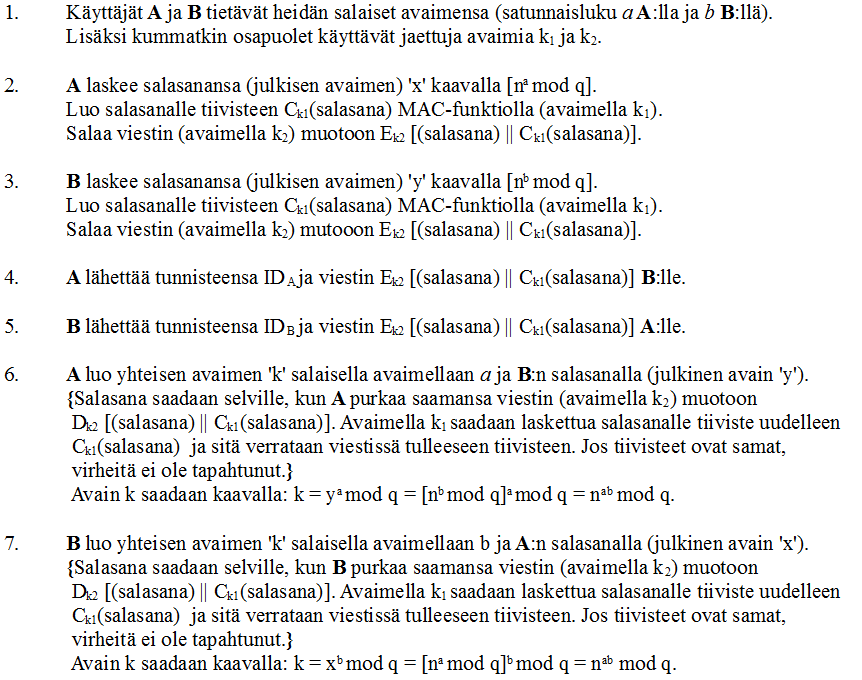
\includegraphics[width=\textwidth]{algoritmis}
\caption{Istuntoavaimen luominen MAC-funktiolla \cite{MAC}}
\end{figure}	

Yhteisiä avaimia ovat aluksi siis 'k1' ja 'k2', joilla viestien vaihtoa suoritetaan. Myöhemmin laskettu 'k' korvaa nämä avaimet. MAC-funktiolla tässä tapauksessa lasketaan tiiviste julkisille avaimille ja funktiossa käytetään yhteisenä salaisuutena avainta 'k1'.


\subsection{Mobiilikaupankäynti}

Mobiilikaupankäynnillä tarkoitetaan mobiililaitteella tehtäviä maksutransaktioita tai ostotapahtuman vahvistavia viestejä. Menetelmä on siis osa elektronista kaupankäyntiä, jossa käytetään digitaalisia allekirjoituksia \cite{e-c}. Schwab ja Yang toteavat  \cite{enti} mobiililaitteilla henkilökohtaisen, rahallisen ja kaupallisen datan varastoinnin olevan yleisessä käytössä. Samadanin, Shajarin ja Ahanihan artikkelissa \cite{proxy} esitellään huutokauppasovellus, joka vaatii jokaisen huudon varmistuksen lyhyen ajan sisällä laitteella. Allekirjoitusten luonti tulee olla siis nopeaa mobiililaitteilla tietoturva huomioon ottaen. Sekä laite- että palvelinpohjaisia allekirjoituksia käytetään mobiilikaupankäynnissä \cite{proxy}. Verkkopankki, maksusuoritukset, terveydenhoito ja äänestys ovat mahdollisia kannettavilla laitteilla, mutta langaton verkko tuo ongelmansa kaistan leveydessä \cite{ECC}. 



\section{Laitepohjaiset allekirjoitukset}

Mobiililaite koostuu SIM-kortista ja laitteesta, jossa allekirjoituksen luonti tapahtuu prosessorilla. Laitteen käyttöjärjestelmän on tuettava yleisesti käytettyjä protokollia, jotta salaus, tiivistefunktiot, varmenteet ja digitaaliset allekirjoitukset ovat mahdollisia. Tietoturvan kannalta SIM-korttia voidaan pitää parempana vaihtoehtona, mutta allekirjoitusten luomisen nopeudessa prosessori on tehokkaampi. Salaisen avaimen säilytyspaikka tulee kuitenkin valita turvallisesti, jotta ulkopuolinen tunkeutuja ei saa tietää salaista avainta. Lisäksi on olemassa malli, jossa SIM-kortti ja laitteen prosessori yhdessä osallistuvat allekirjoituksen luontiin (hybridimalli). Seuraavat alaotsikot perustuvat Samadanin, Shajarin ja Ahanihan malleihin \cite{proxy}. 
 
\subsection{SIM-kortilta luonti}

Laitteen SIM-korttia voidaan pitää turvallisimpana paikkana säilyttää salaista avainta. Edes käyttäjä itse tai laitteen käyttöjärjestelmä ei pääse käsiksi salaiseen avaimeen kortilla. Kuitenkin SIM-kortin laskentakapasiteetti on huomattavasti alhaisempi kuin laitteen prosessorin. Allekirjoituksen luonti SIM-kortilla on erittäin hidasta.   

\subsection{Laitteen prosessorilla luonti}

Salaisen avaimen säilytys voi tapahtua myös laitteen muistissa. Digitaalinen allekirjoitus luodaan tällöin laitteen prosessorilla, joka on laskentateholtaan huomattavasti tehokkaampi kuin SIM-kortti. Käyttöjärjestelmä voi myös tarjota kirjastoja ja työkaluja allekirjoitusten luontiin. Laitteen käyttöjärjestelmässä voi kuitenkin olla tietoturva-aukko, jota hyväksikäyttäen tunkeutujat voivat saada haltuunsa käyttäjän salaisen avaimen.

\subsection{Hybridimalli}

Hybridimallissa salainen avain joudutaan hetkellisesti paljastamaan laitteen käyttöjärjestelmälle. Tässä menetelmässä on siis olemassa pieni tietoturvariski. Hyvänä puolena hybridimallissa on sen lähes yhtä nopea tehokkuus kuin prosessorilla luonnissa. Monet graafisen käyttöliitymän vaativat ohjelmat tarvitsevat prosessorin laskentatehoa, mutta SIM-kortti voi toimia tietoturvan kannalta avaimen yleisenä säilytyspaikkana. Mallissa allekirjoitus siis luodaan prosessorilla, jolloin salaista avainta käytetään vain hetkellisesti laitteessa.


\section{Palvelinpohjaiset allekirjoitukset}

Palvelin voi luoda digitaalisen allekirjoituksen käyttäjän puolesta, kunhan käyttäjä voidaan todentaa palvelimelle. Palvelinten rooli digitaalisten allekirjoitusten luonnissa oli merkittävä aikana, jolloin laitteissa ei ollut tarpeeksi tehoa allekirjoituksen luomiseen. Nykyään laitepohjaiset allekirjoitukset ovat yleistyneet. \cite{proxy}

\subsection{Välityspalvelin}

Välityspalvelin toimii siis eräänlaisena kirjautumispalvelimena käyttäjän ja lopullisen palveluntarjoajan välissä. Välityspalvelin voi luoda allekirjoituksen, mutta oikean käyttäjän todennus vaaditaan. Varmennus voi perustua algoritmeihin kuten RSA tai DSA. On myös mahdollista, että käyttäjälle tehdään varmenne, jolla hän on tunnistettavissa jatkossa palvelimelle \cite{proxy}.

\subsection{NRS ja NRR}

Kiistämättömyys on olennainen osa digitaalista allekirjoitusta. NRS (Non-Repudation of Sender) tarkoittaa, lähettäjä ei voi jälkikäteen kiistää lähettäneensä viestin. NRR (Non-Repudation of Receiver) puolestaan merkitsee vastaanottajan kiistämättömyyttä. Tiivistefunktioilla varmistetaan datan eheys kuten esimerkiksi MD5:llä. Sekä lähettäjän että vastaanottajan on luotava julkiset avaimet ja merkit kirjautumispalvelimelle tunnistettavaksi. Kirjautumispalvelin pyytää varmenteen varmenneviranomaiselta ja muodostaa oman varmenteen lähettäjälle. Näin ollen kirjautumispalvelin voi jatkossa toimia pysyvämpänä vahvistajana lähettäjän ja vastaanottajan välillä. \cite{gene}

\subsection{Yhdistetty allekirjoitus}

Laitteella pystyy delegoimaan allekirjoituksen luonnin palvelimelle kokonaan, osittain tai valtakirjalla. Välityspalvelin voi kokonaan luoda allekirjoituksen käyttäjän salaisella avaimella. Tämä tyyppi ei ole tietoturvan kannalta suotavaa. Osittaisessa allekirjoituksessa käyttäjä luo omasta salaisesta avaimestaan välityspalvelimelle uuden avaimen. Välityspalvelimella on tällöin mahdollisuus tehdä allekirjoitus käyttäjän puolesta. Kiistattomuus nousee näissä kahdessa menetelmässä ongelmaksi. Vastaanottaja ei voi tietää, onko allekirjoitus tullut välityspalvelimelta vai käyttäjältä. Kolmas menetelmä on valtakirjan luovuttaminen välityspalvelimelle. Käyttäjä siis kertoo valtakirjallaan luovuttaneensa allekirjoitusoikeuden toiselle palvelimelle. Valtakirja luodaan käyttäjän salaisella avaimella. Valtakirjan laatiminen saattaa viedä huomattavasti aikaa ja paljon laskentatehoa. \cite{joint}

\subsection{Protokollapyynnöt}

Kun viestiä lähetetään välitys- tai vastaanottajapalvelimelle, on muistettava käyttää protokollan mukaisia pyyntöjä ja vastauksia. Laitteiden ja palvelinten välillä protokollia tulee noudattaa. He ja Zhang \cite{joint} esittelevät kaksi funktiota, joita käytetään yhdistetyssä allekirjoituksessa käyttäjän, välityspalvelimen ja vastaanottajapalvelimen välisessä kommunikaatiossa. Salausavaimeen perustuva MAC-funktio eli HMAC-funktio (Hash Message Authentication Code) varmistaa tiedon eheyden ja viestin todennuksen. Lisäksi voidaan käyttää HOAC-funktiota (Hash Origin Authentication Code), joka toimii HMAC-funktion tapaan. Käyttäjä MS lähettää viestin $m$, joka on allekirjoitettu HOAC-funktiolla. Tälle allekirjoitettulle tiivisteelle luodaan vielä uusi tiedon eheyttä varmistava tiiviste HMAC-funktiolla. Nämä kaikki kolme tiivistettä (m, HOAC ja HMAC) välityspalvelin HE allekirjoittaa uudelleen omalla salaisella avaimellaan. Lopullinen palvelin verifioi kaikki tiivisteet ja saa tiedon, että viesti $m$ kulki käyttäjältä MS välityspalvelimen HE kautta. HOAC-funktio varmistaa viestin lähteneen käyttäjältä MS eli kiistämättömyyden.

\subsection{Tekstiviestitodennus}

Langattomien lähiverkkotekniikoiden yleistymisestä huolimatta tekstiviestillä (SMS) voidaan todentaa käyttäjä. Tarvitaan vain terminaaliemulaattori (T) käyttäjän laitteelle ja turvallinen yhteydenmuodostusportti (GW) kommunikaatiota varten. Terminaali voi olla laitteella erillinen ohjelma tai suoraan integroitu SIM-kortilla oleviin työkaluihin. GW koostuu todennuspalvelimesta ja tietokantapalvelimesta. Todennuspalvelin varmistaa oikean ohjelman käyttävän palvelua ja tietokantapalvelin hallinnoi käyttäjän julkista avainta sekä GW:n salaista avainta.

Seuraavaksi esitelty kuva perustuu Shun, Tanin ja Wangin \cite{sms} tutkimuksiin turvallisesta mobiilikäyttäjän todentamisesta. Sekä T:n että GW:n on luotava tunnistemuuttuja (VF), jolla osapuolet todentavat toisensa. Muuttuja voi olla esimerkiksi tietyn pituinen tiiviste, joka perustuu satunnaislukuihin. Lähtevät paketit luonnollisesti salataan. Oletetaan tiivisteen nimeksi vaikka Nc. Terminaali tekee yhteydenmuodostuspyynnön REQ1, jossa on mukana Nc. GW tutkii pyynnön ja tarkistaa käyttäjän identiteetin sekä puhelinnumeron. Tietokantakyselyllä GW varmistaa käyttäjän löytyvän tietokannasta. GW luo oman VF:n nimeltä Ns ja istuntoavaimen nimeltä Ks. Nämä molemmat muuttujat sekä aiemman Nc:n GW allekirjoittaa salaisella avaimellaan. ACK1-vastauksessa GW hyväksyy yhteydenmuodostuksen ja lähettää salatussa muodossa Nc:n, Ns:sän ja Ks:sän. Tämän jälkeen T:llä allekirjoitetaan saapunut ACK1-vastaus käyttäjän laitteessa olevalla salaisella avaimella. Jos allekirjoitettu Nc' on sama kuin käyttäjän alunperin lähettämä Nc-muuttuja, T salaa Ks:sän ja Ns:sän uudessa pyyntöviestissä REQ2 ja suorittaa lähetyksen. Nyt puolestaan GW allekirjoittaa Ns:n. Mikäli Ns' on sama kuin alunperin lähetetty Ns, yhteys käyttäjän ja palvelimen välille on luotu ja GW lähettää terminaalille kuittauksen ACK2 yhteydenmuodostuksen onnistumisesta. Alla oleva kuva kertoo tarkemmin protokollasta.   

\begin{figure}[h!]
\centering
	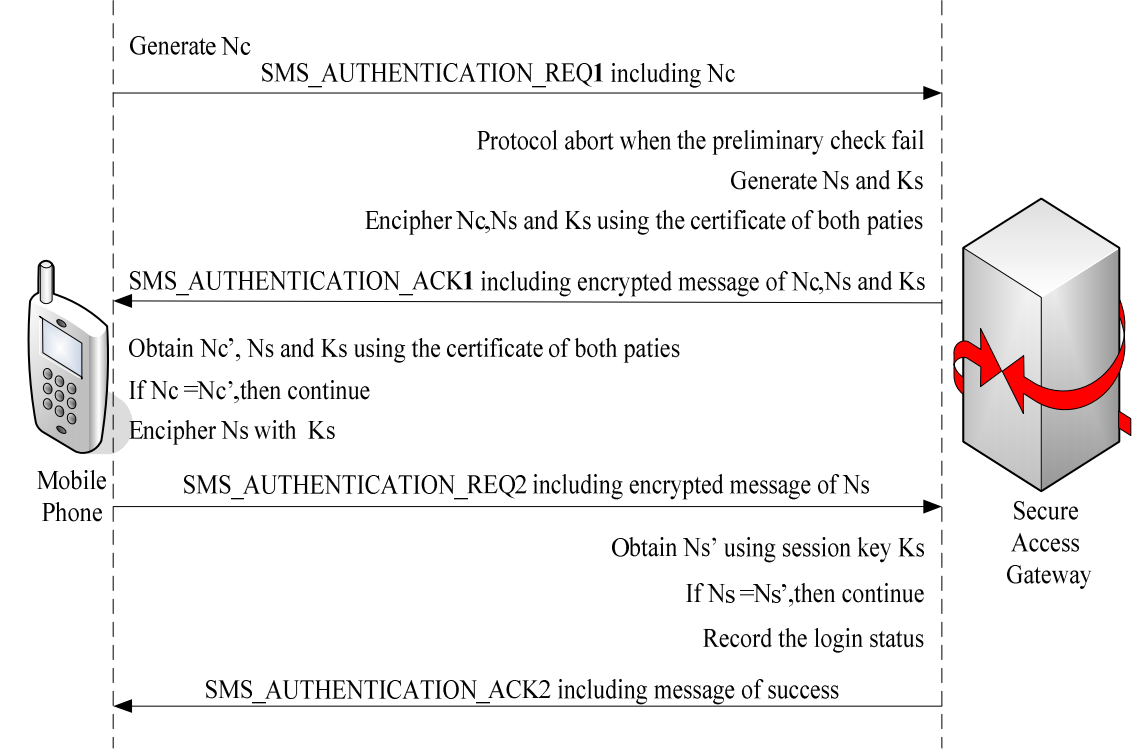
\includegraphics[scale=0.39]{sms-todennus}
\caption{SMS-todennus \cite{sms}}
\end{figure}

Koska protokolla perustuu satunnaisiin muuttujiin, se on resistanssi välimieshyökkäykselle. Myös kiistämättömyys luodaan, sillä käyttäjän salainen avain säilyy vain laitteessa, ja ainoastaan terminaali käyttää avainta. Tätä kyseistä protokollaa voidaan siis pitää yhdistettynä mallina palvelin- ja laitepohjaisesta allekirjoituksesta.


\section{Turvallinen etäyhteys}

On tilanteita, joissa käyttäjä haluaa muodostaa suoran yhteyden palvelimelle tai toiseen tietokoneeseen. Tällöin jatkuva viestien todentaminen osapuolten välillä käy rasittavaksi. Sen sijaan tiedon salausta on korostettava, ja käytettävän verkon turvallisuudesta huolehdittava. Mobiililaitteen ja palvelimen välille voidaan muodostaa virtuaalinen erillisverkko (VPN), jossa käyttäjä tunnistautuu palveluntarjoajalle erillisen VPN-palvelimen avulla. Osapuolten on sovittava yhteisistä standardeista ja protokollista yhteyden muodostamisen ajaksi.

\subsection{Salattu VPN-yhteys}

Yu, Chen ja Tan \cite{vpn} esittelevät turvallisen käytännön mobiililaitteelle muodostaa VPN-yhteys käyttäen SSL-salausta (Secure Sockets Layer). Täytyy kuitenkin huomata kyseessä olevan nykyaikainen turvallisempi TLS-salaus (Transport Layer Security), jota kutsutaan vain yleensä SSL:ksi. SSL:llään kuuluu paljon protokollia, joissa esimerkiksi vaihdetaan salaisia parametreja, luodaan salausavain ja käytetään X.509-varmenteita. Mobiililaitteella tunnistaudutaan VPN SSL- palvelimelle, minkä jälkeen yhteys palveluntarjoajalle muodostetaan palvelimen toimesta. Käyttäjän ei siis tarvitse tunnistautua vielä erikseen palveluntarjoalle tässä tapauksessa. Alla oleva kuva havainnollistaa yhteyden muodostamista asiakkaan ja palveluntarjoajan välillä.

 
\begin{figure}[h!]
\centering
	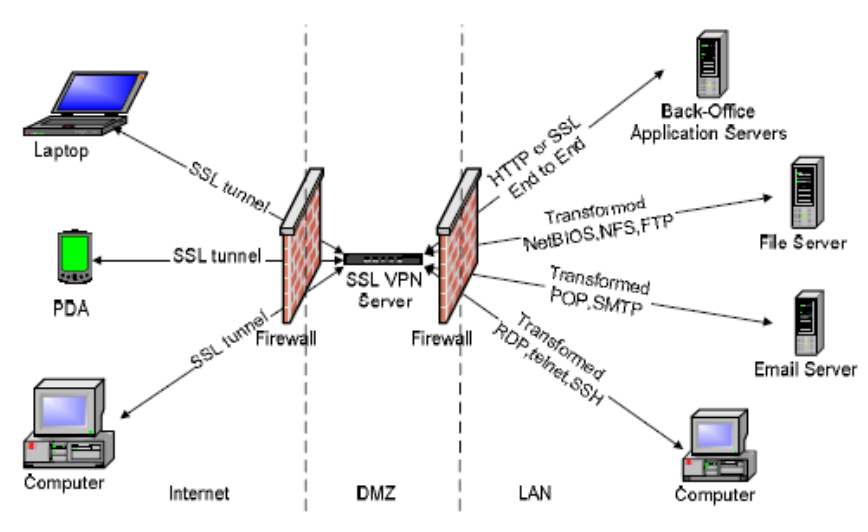
\includegraphics[scale=0.47]{VPN-tunneli}
\caption{VPN-yhteys laitteelta palvelimelle \cite{vpn}}
\end{figure}	

Mobiililaitteella tulee olla työkalut VPN-yhteyden, varmenteiden ja SIM-kortin hallintaan. Lisäksi salauksen/purkamisen asetuksia on päästävä muuntamaan. VPN-palvelimella on turvallisuusjärjestelmä (SAS), jossa on työkalut portin yhteysasetuksiin, yhteys varmenneviranomaisiin, salaus- tai purkuasetukset ja käyttäjätileihin liittyvät hallintamekanismit. VPN-yhteys muodostetaan käyttäjän terminaalin ja  VPN-portin välille. Palveluntarjoajalla ja VPN-palvelimella on omat protokollat yhteyttänsä varten.

VPN-yhteyden voi muodostaa käyttäen WLAN:ia tai GPRS:ää. Käyttäjän yhteydenmuodostuspyynnöt VPN-porttiin muistuttavat TCP-protokollaa (Transmission Control Protocol). Istuntoa varten sovitaan protokollien versoista, istunnon tunnisteesta, salausavaimesta ja käytettävistä funktioista. SSL-yhteys luodaan, kun käyttäjä on todennettu VPN-palvelimen turvallisuusjärjestelmän avulla. Seuraavaksi tarkastetaan käyttäjän oikeudet palveluun. Palveluntarjoaja antaa tarvittavan ohjelmatiedon käyttäjälle VPN-palvelimen vahvistettua käyttäjäoikeudet. Kaikki tieto käyttäjän ja VPN-palvelimen välillä kulkee salattuina paketteina. Jatkuva suojattu yhteys mahdollistaa huipputurvallisuutta vaativien sovellusten kuten verkkopankin käytön mobiiliympäristössä.

\section{Käyttäjän todennus}

Viestien todennusten lisäksi on tärkeää varmistaa oikean käyttäjän käyttävän laitetta. Luonnollisesti on keksittävä keino todentamiseen, jossa vain käyttäjä tietää salaisuuden päästäkseen hallitsemaan laitetta tai lähettääkseen viestin. Schlöglhoferin ja Sametingerin \cite{secure} artikkelissa mainitaan mahdollisiksi todennustavoiksi PIN-koodi, salasana ja kosketuksella tunnistaminen. Tietoturvauhaksi mainitaan laitteen kadottaminen ja päätyminen väärälle käyttäjälle. Tietämykseen perustuvat tunnistamiset ovat vain oikean käyttäjän tiedossa, mutta pätevää tunnistautumista tässä tapauksessa ei voida liittää oikeaan käyttäjään. Myös hyökkääjällä on mahdollisuus arvata pätevä salasana riippuen hyväksyttyjen yritysten määrästä. Todennukset voivat perustua muuhunkin kuin oikean vastauksen tietämykseen. Uusia menetelmiä ovat elektroniset NFC-tarrat ja kameralla otettava kuva. Androidille on tarjolla sovellus nimeltä SecureLock. Sillä voi valita erilaisia tapoja todentaa käyttäjä laitteelle. 

\subsection{PIN-koodi ja salasanatodennus}

PIN-koodi ja salasana ovat yleisesti käytettyjä tunnistautumismenetelmiä. SIM-kortille todennus tapahtuu PIN-koodilla, joka voi olla käyttäjän tai verkko-operaattorin määrittelemä. Salasanalla tunnistaudutaan osaltaan laitteelle. SecureLock-sovelluksessa kuitenkin salasana voi olla pituudeltaan rajoittamaton. Salasanassa voi olla isoja ja pieniä kirjaimia ja lisäksi sisältää erikoismerkkejä.   Lisäksi on olemassa PUK-koodi (Personal unblocking code), joka voidaan syöttää laitteeseen PIN-koodin tai muun todennustavan unohduttua.

\subsection{Kosketustodennus}

Kosketustodennukseen kuuluu graafisen salasanan syöttäminen. SecureLock tarjoaa kosketustunnistautumisen, jossa käyttäjä rajaa sormenliikkeellään tietyn alueen laitteen ruudulta. Tähän ruutuun täytyy lisäksi sisältyä tietty määrä symboleita, jotka voivat olla esimerkiksi hedelmiä. Alla olevassa kuvassa keltainen neliö on rajattu alue, jolta täytyy löytyä sateenvarjon, suklaamuffinssin ja mansikan kuvakkeet. Käyttäjä piirtää valitsemansa alueen kosketusnäytöllä. Alueen on oltava myös oikean kokoinen, jotta todennus hyväksytään. Tässä tunnistautumistavassa yhdistyvät käyttäjän tietämys oikean alueen koosta, sijainnista ja tarvittavista symboleista.


\begin{figure}[h!]
\centering
	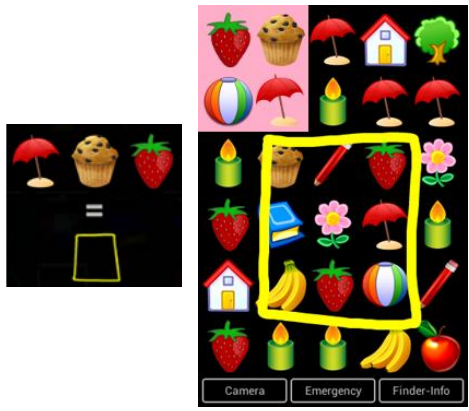
\includegraphics[scale=0.5]{gesture}
\caption{Käyttäjän todentaminen SecureLockilla \cite{secure}}
\end{figure}

\subsection{Muita todennustapoja}

NFC on uusi teknologia, joka tarjoaa elektronisten tarrojen avulla tunnistautumisen laitteelle. Laite lukee tarrasta koodin, joka mahdollistaa todennuksen. Tarroja voi olla useampi ja laitteen on teknisiltä ominaisuuksiltaan tuettava NFC-todennusta. Laitteen kameralla on lisäksi mahdollisuus tunnistautua. Kuvan voi ottaa ilman tunnistautumista, mutta aikaisempia otettuja kuvia ei pysty tarkastelemaan laitteella. Kuvan kohteena voisivat toimia omat kasvot tai henkilökortti. Näin ollen käyttäjän tarvitse muistaa vain kohde, jota tarvitaan todennukseen.

\subsection{Tunnistautuminen GSM-verkossa}

Langattomassa verkossa on tärkeää, että viestin lähettäjä tietää lähettävänsä viestin oikealle kohteelle ja vastaanottaja tietää saavansa viestin oikealta lähettäjältä. Osapuolten sijainti ja aikaleimat saattavat muuttua viestien vaihdon aikana. Jaiswal ja Kumar \cite{cell} esittelevät GSM-verkon toimintaa kahden mobiililaitteen käyttäjän näkökulmasta. Tähän väliin tarvitaan pääsolmu, joka luo yhteisen avaimen osapuolille viestien vaihtoa varten. Verkko voidaan jakaa useampaan kenttään, jossa jokaisessa on oltava vähintään yksi pääsolmu laitteiden tunnistautumista varten. Pääsolmun on tiedettävä kaikki oman kenttänsä laitteet ja muita pääsolmuja tiedon vaihtoa varten. Pääsolmun luo yhteisen avaimen osapuolille tulevaa tiedonvaihtoa varten tunnistetietojen perusteella. Pääsolmu tarvitsee laitteilta tärkeät tiedot tunnistamiseen parametrien ja sijainnin avulla. Alla oleva kuva kertoo GSM-verkon rakennetta tarkemmin.

\begin{figure}[h!]
\centering
	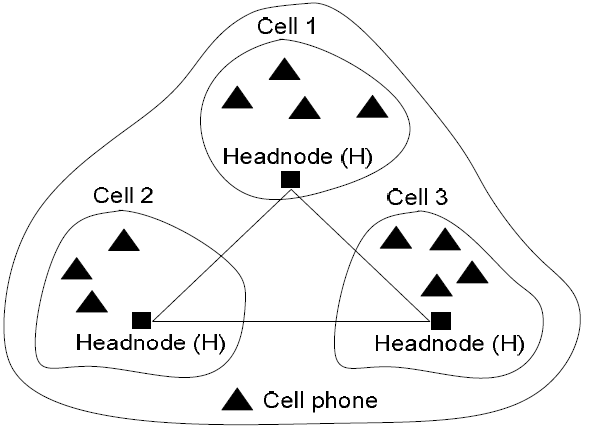
\includegraphics[scale=0.6]{nodes}
\caption{Langattoman verkon solmujen rakenne \cite{cell}}
\end{figure}	

Laitteiden on siis lähetettävä viesteissä parametreina tarvittavat tiedot aina solmulta solmulle. Tiedonkeruun jälkeen pääsolmu luo yhteisen avaimen osapuolille tulevaa kommunikaatiota varten. Avaimella voi hoitaa viestien salauksen ja tiivisteen käytön. Koko yhteyden aikana on päivitettävä tunnistetietoja solmuille.

\section{Vertailu}

Tehokkuus ja tietoturva ovat tärkeitä ominaisuuksia koskien digitaalisia todennuksia. Vaikka nämä kaksi seikkaa eivät ole suoraan toisensa poissulkevia, on syytä ottaa huomioon kummankin prioriteetti. Digitaalinen allekirjoitus vaatii enemmän tehokkuutta kuin MAC-funktio tai DH pidempien avainten ja varmenteen liittämisen takia. Tietoturvaltaan sen sijaan digitaalinen allekirjoitus on parempi sen lähettäjän kiistämättömyyden takia. Erityisesti mobiililaitteilla tehokkuudesta joudutaan yleensä karsimaan, joten valitaan vähemmän tehokas allekirjoitusalgoritmi. Tällöin allekirjoittaminen on hidas prosessi \cite{proxy}.

\subsection{Tietoturva}

Mobiililaitteilla voidaan havaita seuraavia tietoturvariskejä: urkinta, välimieshyökkäys, datan muuntaminen, toisena osapuolena esiintyminen ja laitteen kadottaminen. Urkinnalla tarkoitetaan viestien kuuntelua, mutta se voidaan torjua helposti viestin salakirjoituksella esimerkiksi väliaikaisen istuntoavaimen avulla. Välimieshyökkäys tarkoittaa kolmannen osapuolen asettumista lähettävän ja vastaanottavan osapuolten väliin. DH:n perusversiossa voi piileä tämä riski mutta ei yleensä RSA:ssa \cite{enti}. Datan muuntaminen voidaan estää erilaisilla salausmenetelmillä sekä käyttämällä tiivisteitä. Toisena osapuolena tekeytyminen ja laitteen kadottaminen voidaan estää salasanan kirjoittamisella laitteelle tai visuaalisella todennuksella kuvion piirtämisellä. 

Julkisen avaimen infrastruktuuri eli PKI-malli toimii, jos salainen avain säilyy suojassa. Mikäli on pienikin riski, että salainen avain on jokun muun tiedossa tulee avainpari vaihtaa heti. Sama riski koskee symmetrisen salauksen avaimia MAC-funktiossa ja DH:ssa. Niin kauan kun diskreetin logaritmin ongelmaa ei pystytä ratkaisemaan toteuttamiskelpoisessa ajassa, ovat RSA ja DH turvallisia protokollia. Tiivistefunktioiden vaatimusten tulee olla myös ajan tasalla, jotta tiivisteistä ei pystytä päättelemään tekstin rakennetta. Esimerkiksi tulevaa SHA-3 standardia kehitellään paremmaksi tulevaa käyttöönottoa varten \cite{nist}. AES salausalgoritmia voidaan pitää murtumattomana, mutta DSA on murrettavissa jo muutaman bittivuodon avulla \cite{gsm}. Salausalgoritmeista ei saa olla pääteltävissä salatun tekstin yhteys selväkieliseen tekstiin ja yhden bitin diffuusion tulee vaikuttaa useampaan bittiin.

Riskit mobiiliympäristössä ovat kasvaneet viime aikoina. Mobiililaitteilla on suuret riskit tietoturvahyökkäyksille langattoman verkon käytön takia. Vuonna 2012 Android-alustalle oli yli 200 000 erilaista sovellusta Adroid Marketissa. Yli 250 000 Android-sovellusten käyttäjää ilmoitti ladanneensa haitallisen ohjelman, joka vaikutti aluksi luotettavalta. \cite{enti}

Laitepohjaiset allekirjoitukset ovat vakiintuneet kokoajan mobiililaitteiden laskentatehon kasvun ansiosta. RSA:n lisäksi elliptiset käyrät ovat yleistyneet niiden paremman tietoturvan ansiosta suhteessa avainten pituuteen bitteinä \cite{ECC}. Elliptisen käyrän DSA:ta käytetään myös mobiililaitteilla \cite{webs}. RSA:n avaimen pituuden on hyvä olla vähintään 1024 bittiä. Elliptisissä käyrissä riittää 160 bittiä tällä hetkellä \cite{ECC}.   
	  

\subsection{Tehokkuus}

Suorituskyky on parantunut vuosien saatossa niin tietokoneilla kuin mobiililaitteilla. Vielä vuonna 2004 uskottiin matkapuhelinten ja kämmentietokoneiden laskentatehon olevan liian riittämättömiä digitaalisiin allekirjoituksiin \cite{gene}. Kuitenkin vuonna 2012 julkisen avaimen infrastruktuurin siirtämisen tarve kokonaan mobiilialustoille muuttui ajankohtaiseksi aiheeksi \cite{ECC}. Prosessorien teknologia on kehittynyt mahdollistaen tiheämmät kellopulssit ja moniydinsuorituksen. Myös tietoliikennenopeuksien kasvamisella on ollut suuri merkitys digitaalisten allekirjoitusten luonnissa ja muissa todennustavoissa. Tehokkuutta tarvitaan nopeisiin allekirjoituksiin lyhyellä aikavälillä. Artikkelissa Self-Proxy Mobile Signature \cite{proxy} esitelty huutokauppasovellus tarvitsee jokaiselle huudolle uuden  allekirjoituksen lyhyen ajan sisällä. Tietoturvasta on tässä tapauksessa erittäin vaikea tinkiä, joten käyttäjän olisi hyvä luoda allekirjoitus omalta laitteeltaan. Tehokkuudessa tulee ottaa huomioon siis salauksen nopeus, tiivisteen luominen ja varmenteen hankinta \cite{proxy}. Luonnollisesti myös palvelinpuolella esimerkiksi klusterointi on luonut mahdollisuuden tehokkaaseen allekirjoitusten/varmenteiden luomiseen monelle käyttäjälle samaan aikaan.

Salauksella on suuri merkitys tehokkuudessa. On aivan eri asia salata pelkkä tiiviste kuin koko viesti. Aikaisemmin esitelty Saxenan ja Chaudharin \cite{gsm} tutkimus osoittaa eroja salausalgoritmien välillä mobiililaitteissa perustuen salaustekniikkaan ja avainten kokoon. Rayn ja Biswasin \cite{ECC} tutkimuksessa elliptisten käyrien käyttö osoittautui tehokkaammaksi kuin RSA mobiilisovelluksissa. Xuanin, Dun ja Chenin \cite{webs} tutkimuksessa havaittiin 512-bittiä pitkän avaimen RSA:ssa ja 600-bittiä pitkän avaimen elliptisissä käyrissä aikaeroksi miljardien konekäskyjen ero.

Yhteydenmuodostuksen nopeus on tärkeä asia turvallisessa verkkoyhteydessä. Yun, Chengin ja Tanin \cite{vpn} tutkimuksessa VPN-yhteyden luomisessa kesti GRPS-verkossa 8,1 sekuntia. WLAN puolestaan suoritti saman yhteyden muodostamisen 3,2 sekunnin ajassa. Verkon tyypillä on siis suuri merkitys todennusten nopeudessa, joten mobiililaitteiden laskentatehon parantaminen ei ole ainoa keino kehittää tehokasta todennusta käyttäjän näkökulmasta.   


\subsection{Sovellusten kehittäminen}

Android-käyttöjärjestelmä tukee Javan virtuaalikonetta (JVM). Java käyttää digitaaliseen allekirjoitukseen tarvittavia protokollia, joita tarvitaan monilla mobiililaitteilla nykypäivänä. Bouncy Castle- paketti tarjoaa Javassa monenlaista kryptografisia algoritmeja tiedon salaukseen ja purkamiseen. Javalla myös satunnaisten olioiden luominen on helppoa. \cite{enti}

Tuotteille joiden käyttöjärjestelmänä on Applen iOS, on julkaistu Common-Crypto-rajapinta. Se sisältää erilaisia tiiviste- ja salausalgoritmeja sovellusten kehittämiseen. Tehokkuus on otettu huomioon API:n ominaisuuksissa. Ohjelmointikielistä C on tuettu, ja algoritmit painottuvat symmetrisiin salauksiin. \cite{ios}

Microsoftin Windows-käyttöjärjestelmä on siirtynyt mobiiliyhteensopivaksi viime vuosina. CryptoAPI on kirjasto, joka 	toimii ohjelmointikielillä C ja C++. Digitaaliset allekirjoitukset ja symmetriset salausmenetelmät ovat tuettuja CryptoAPI:ssa.   Kirjasto on osa Windows Mobile SDK -työkalupakettia, jota voidaan käyttää tietokone- ja mobiililaitteistoilla. \cite{windows}
   

\section{Yhteenveto}  

Tässä tekstissä olemme tarkastelleet digitaalisia todennuksia mobiiliympäristöissä ja mobiililaitteissa. Todennuksiin kuuluvat digitaalinen allekirjoitus, MAC-funktio ja symmetriseen salaukseen perustuva Diffien ja Hellmanin menetelmä. Digitaalisen allekirjoituksen ehtoina ovat vastaanottajan todennus, datan eheys ja lähettäjän kiistämättömyys. Menetelmät allekirjoitusten luontiin ja todennusten käyttöön vastaavat tietokoneilla samanlaisia menetelmiä. Monet digitaaliset todennukset perustuvat vanhoihin algoritmeihin, jotka kehitettiin jo 1970-luvulla. Olemme tarkastelleet matemaattisia menetelmiä, joita tarvitaan RSA:ssa, DH:ssa ja MAC-funktiossa. Digitaalisten allekirjoitusten luonti voidaan jakaa kahteen pääryhmään: laite- ja palvelinpohjaisiin allekirjoituksiin. Laiteella allekirjoituksen voi luoda prosessori tai SIM-kortti. Lisäksi hybridimallin olemassaolo tunnetaan. Palvelinpuolella tulee korostua käyttäjän tunnistaminen ja kirjautumispalvelimen merkitys. Palvelimelle on osattava myös lähettää viestit ja muodostaa yhteys tiettyjen protokollapyyntöjen avulla. Kiistattomuuden tulee toimia delegoinnin yhteydessä. Digitaalinen allekirjoitus voidaan delegoida palvelimelle kokonaan, osittain tai valtakirjalla. Varmenteet ja kiistattomuus luovat digitaalisen allekirjoituksen pohjan. Olemme tarkastelleet tekstin lopussa tietoturvan ja tehokkuuden merkitystä digitaalisissa todennuksissa mobiililaitteiden näkökulma huomioon ottaen. Nykyaikaisiin menetelmiin voimme luetella RSA:n, DH:n ja MAC-funktioiden lisäksi elliptiset käyrät. Näitä algoritmeja tukevia käyttöjärjestelmiä ovat Android, iOS ja Windows. Erilaisten salausmenetelmien ja verkkotekniikoiden käytöllä on vaikutusta todennusten tehokkuuteen ajallisesti. Käyttöjärjestelmille luodut API-kirjastot auttavat ohjelmistojen kehittäjiä luomaan mobiilialustoille yhteensopivia ohjelmistoja. Sovellusten jatkuva suosio asettaa korkeat tavoitteet niin tietoturvalle kuin tehokkuudelle.

% --- References ---
%
% bibtex is used to generate the bibliography. The babplain style
% will generate numeric references (e.g. [1]) appropriate for theoretical
% computer science. If you need alphanumeric references (e.g [Tur90]), use
%
% bibliographystyle{babplain-lf}
%
% instead.

\newpage
\bibliographystyle{babalpha-lf}
\bibliography{viitteet}


% --- Appendices ---

% uncomment the following

%\newpage
%\appendix
 
%\section{Esimerkkiliite}

\end{document}